\باب{فوریئر تجزیہ}
\اصطلاح{دوری تفاعل}\فرہنگ{دوری!تفاعل}\فرہنگ{تفاعل!دوری}\حاشیہب{periodic function}\فرہنگ{periodic!function} سے مراد وہ تفاعل ہے جو درج ذیل مساوات پر پورا اترتا ہے
\begin{align}
f(t)=f(t+nT_0), \quad n=\mp 1, \mp 2, \mp3, \cdots
\end{align}
جہاں \عددی{T_0}  \اصطلاح{دوری عرصہ}\فرہنگ{دوری عرصہ}\حاشیہب{time period}\فرہنگ{time period} کہلاتا ہے۔شکل \حوالہ{شکل_فوریئر_چند_دوری_امواج} میں چند \اصطلاح{دوری امواج}\فرہنگ{دوری!موج}\فرہنگ{موج!دوری}\حاشیہب{periodic wave}\فرہنگ{periodic!wave} دکھائے گئے ہیں۔
\begin{figure}
\centering
\begin{subfigure}{0.5\textwidth}
\centering
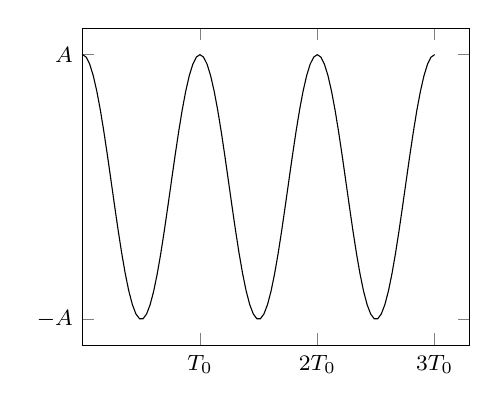
\begin{tikzpicture}
\begin{axis}[small,xmin=0,xtick={360,720,1080},xticklabels={$T_0$, $2T_0$,$3T_0$},ytick={-1,1},yticklabels={$-A$,$A$}]
\addplot[domain=0:1080,samples=100]{cos(x)};
\end{axis}
\end{tikzpicture}
\caption*{(الف) سائن نما موج۔}
\end{subfigure}%
\begin{subfigure}{0.5\textwidth}
\centering
\begin{tikzpicture}
\begin{axis}[small,xmin=0,xtick={1,3,6},xticklabels={$T_a$, $T_0$,$2T_0$},ytick={1},yticklabels={$A$}]
\addplot[] plot coordinates {(0,0) (0,1) (1,1) (1,0) (3,0) (3,1) (4,1) (4,0)(6,0) (6,1) (7,1) (7,0)};
\end{axis}%
\end{tikzpicture}
\caption*{(ب) مستطیل موج۔}
\end{subfigure}
\begin{subfigure}{0.5\textwidth}
\centering
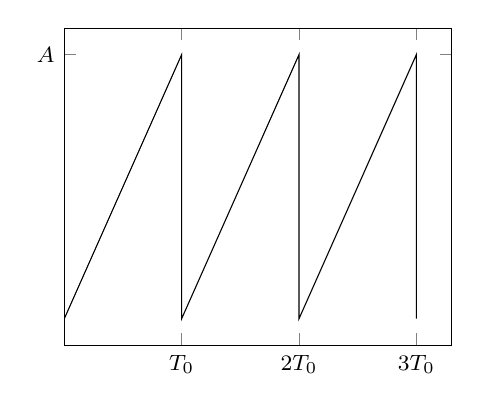
\begin{tikzpicture}
\begin{axis}[small,xmin=0,xtick={3,6,9},xticklabels={$T_0$, $2T_0$,$3T_0$},ytick={1},yticklabels={$A$}]
\addplot[] plot coordinates {(0,0) (3,1) (3,0) (6,1) (6,0) (9,1) (9,0)};
\end{axis}%
\end{tikzpicture}
\caption*{(پ) دندان موج۔}
\end{subfigure}%
\begin{subfigure}{0.5\textwidth}
\centering
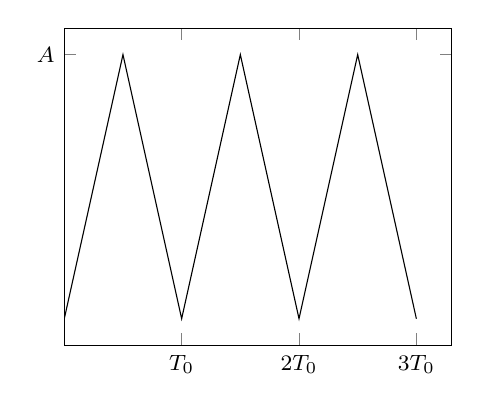
\begin{tikzpicture}
\begin{axis}[small,xmin=0,xtick={2,4,6},xticklabels={$T_0$, $2T_0$,$3T_0$},ytick={1},yticklabels={$A$}]
\addplot[] plot coordinates {(0,0) (1,1) (2,0) (3,1) (4,0) (5,1) (6,0)};
\end{axis}%
\end{tikzpicture}
\caption*{(ت) تکونی موج۔}
\end{subfigure}%
\caption{چند دوری امواج۔}
\label{شکل_فوریئر_چند_دوری_امواج}
\end{figure}


